\documentclass[a4paper,12pt]{article}

%%% Работа с русским языком
\usepackage{cmap}					% поиск в PDF
\usepackage{mathtext} 				% русские буквы в формулах
\usepackage[T2A]{fontenc}			% кодировка
\usepackage[utf8]{inputenc}			% кодировка исходного текста
\usepackage[english,russian]{babel}	% локализация и переносы
\usepackage{xcolor}
\usepackage{hyperref}
 % Цвета для гиперссылок
\definecolor{linkcolor}{HTML}{799B03} % цвет ссылок
\definecolor{urlcolor}{HTML}{799B03} % цвет гиперссылок

\hypersetup{pdfstartview=FitH,  linkcolor=linkcolor,urlcolor=urlcolor, colorlinks=true}

%%% Дополнительная работа с математикой
\usepackage{amsfonts,amssymb,amsthm,mathtools} % AMS
\usepackage{amsmath}
\usepackage{icomma} % "Умная" запятая: $0,2$ --- число, $0, 2$ --- перечисление

%% Номера формул
%\mathtoolsset{showonlyrefs=true} % Показывать номера только у тех формул, на которые есть \eqref{} в тексте.

%% Шрифты
\usepackage{euscript}	 % Шрифт Евклид
\usepackage{mathrsfs} % Красивый матшрифт

%% Свои команды
\DeclareMathOperator{\sgn}{\mathop{sgn}}

%% Перенос знаков в формулах (по Львовскому)
\newcommand*{\hm}[1]{#1\nobreak\discretionary{}
{\hbox{$\mathsurround=0pt #1$}}{}}
% графика
\usepackage{graphicx}
\graphicspath{{pictures/}}
\DeclareGraphicsExtensions{.pdf,.png,.jpg}
\author{Бурмашев Григорий, БПМИ-208}
\title{ТВиМС, ластовый}
\date{\today}
\begin{document}
\maketitle 
\begin{center}
\textbf{But the very next day you gave it away...}
\end{center}
\clearpage
\begin{center}
\textbf{С НОВЫМ ГОДОМ!}
\end{center}
\begin{center}

\includegraphics[scale=0.3]{5.jpg}
\end{center}
\clearpage
\section*{Номер 3}
Плотности:
\[
\rho_X(t) = I_{\{t \in [0, 1]\}}
\]
\[
\rho_Y(t) = I_{\{t \in [0, 1]\}}
\]
\[
\rho_U(t) = 
\lambda \cdot e^{-\lambda t} \cdot I_{\{t > 0\}}
\]
\[
\rho_V(t) = 
\lambda \cdot e^{-\lambda t} \cdot I_{\{t > 0\}}
\]
\subsection*{f)}
\[
\rho_{X+U}(t) = \int\limits_{-\infty}^{+\infty} \rho_X(z) \rho_U(t-z) dz =
\int\limits_{-\infty}^{+\infty}I_{\{z \in [0, 1]\}} \cdot \lambda \cdot e^{-\lambda (t-z)} \cdot I_{\{(t-z) > 0\}}dz   =
\]
\[
=
\lambda \cdot e^{-\lambda t} 
\int\limits_{-\infty}^{+\infty}I_{\{z \in [0, 1]\}} \cdot \lambda \cdot e^{\lambda z} \cdot I_{\{(t-z) > 0\}}dz 
=
\begin{cases}
0, t < 0 \\
a = \min (1, t) \\
\lambda \cdot e^{-\lambda t} \int\limits_0^{a} e^{\lambda z} dz, t > 0
\end{cases} = 
\]
\[
=
\begin{cases}
0, t < 0 \\
\lambda \cdot e^{-\lambda t} \frac{e^{\lambda \cdot a} -1 }{\lambda}, t > 0, a = \min (1, t)
\end{cases}
=
\begin{cases}
e^{-\lambda t} (e^{\lambda \cdot a} -1) , t > 0, a = \min (1, t) \\
0, \text{иначе}  \\
\end{cases}
\]
\begin{center}
\textbf{Ответ: } 
\[
\rho_{X+U}(t) 
=
\begin{cases}
e^{-\lambda t} (e^{\lambda \cdot a} -1) , t > 0, a = \min (1, t) \\
0, \text{иначе}  \\
\end{cases}
\]
\end{center}
\section*{e)}
По определению:
\[
\rho_{\frac{U}{V}}(t) = F'_{\frac{U}{V}}(t)
\]
Считаем:
\[
F_{\frac{U}{V}} (t) = P\left(\frac{U}{V} \leq t\right) = P((U, V) \in A_t), A_t = \left\{ x \in X, y \in Y : \frac{x}{y} \leq t \right\}
\]
\[
P((U, V) \in A_t) = \iint\limits_{A_t} \lambda e^{- \lambda x} I_{\{x > 0\}} \cdot \lambda e^{- \lambda y} I_{\{y > 0\}} dxdy = \iint\limits_{\begin{matrix}
x \leq ty \\
x > 0 \\
y > 0
\end{matrix}} \lambda^2 e^{-\lambda(x+y)} dx dy =
\]
\[
=
 \begin{cases}
\int\limits_0^{\infty} dy \int\limits_0^{ty} \lambda^2 e^{-\lambda (x + y)} dx \\
0, \text{иначе}  \\
\end{cases}
\]
Посчитаем интеграл отдельно:
\[
\int\limits_0^{\infty} dy \int\limits_0^{ty} \lambda^2 e^{-\lambda (x + y)} dx = \int\limits_0^{\infty}  \cdot \lambda^2 e^{-\lambda y} \cdot \left(-\frac{e^{-\lambda ty} - 1}{\lambda} \right) dy  = \int\limits_0^{\infty}  \lambda e^{-\lambda y} \cdot( -\left(e^{-\lambda ty} - 1 \right)) dy = \]
\[
=
\lambda \int_0^{\infty} \left( e^{-\lambda(1+t)y} - e^{-\lambda y} \right)dy = - \lambda \cdot \left(\frac{1}{\lambda(1+t)} - \frac{1}{\lambda} \right) =- \frac{1}{1+t} + 1
\] 
Возвращаемся к системе, она теперь будет равна:
\[
\begin{cases}
-\frac{1}{t+1} + 1, t > 0\\
0, \text{иначе} \\
\end{cases}
\]
Это была функция распределения, возьмем производную и получим ответ:
\begin{center}
\textbf{Ответ: } 
\[
\rho_{\frac{U}{V}}(t) = \begin{cases}
\frac{1}{(1+t)^2}, t > 0 \\
0, \text{иначе}
\end{cases}
\]
\end{center}
\section*{h)} 
Аналогично:
\[
\rho_{UX}(t) = F'_{UX}(t)
\]
\[
F_{UX}(t) = P(UX \leq t) = \iint\limits_{\begin{matrix}
u \leq \frac{t}{x} \\
x \in [0, 1] \\
u > 0
\end{matrix}} \lambda e^{-\lambda u} du dx 
=\int_0^1 dx \int_0^{\frac{t}{x}} \lambda e^{-\lambda u} du  = 1-  \int_0^1 e^{-\frac{\lambda t}{x}} 
\]
Тогда:
\[
\rho_{UX}(t) =  \begin{cases} -\frac{d}{dt} \int_0^1 e^{\frac{\lambda t}{x}}dx, t > 0 \\
0, \text{иначе}  \end{cases}= \begin{cases} \int\limits_0^1 \frac{\lambda}{x} e^{-\frac{\lambda t}{x}} dx, t > 0\\
0, \text{иначе}
\end{cases}
\]
\begin{center}
\textbf{Ответ: } 
\[
\rho_{UX}(t) = 
\begin{cases} \int\limits_0^1 \frac{\lambda}{x} e^{-\frac{\lambda t}{x}} dx, t > 0\\
0, \text{иначе}
\end{cases}
\]
\end{center}
\clearpage
\section*{Номер 7}
\begin{center}
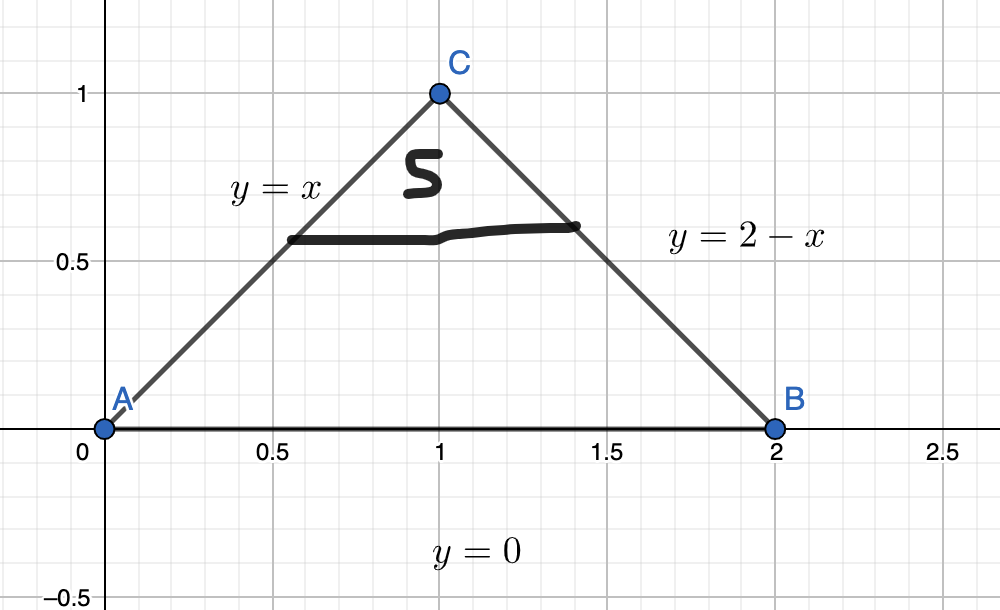
\includegraphics[scale=0.5]{1.png}
\end{center}
\[
P(X \leq x) = F_X(x) = 
\begin{cases}
0, x \in (-\infty, 0] \\
\int\limits_0^x tdt,  x \in (0, 1)\\
\frac12 + \int\limits_1^x (2-t)dt, x \in [1, 2) \\
1, x \in [2, \infty) \\
\end{cases}
=
\begin{cases}
0, x \in (-\infty, 0] \\
\frac{x^2}{2}, x \in (0, 1) \\
-\frac{x^2}{2} + 2(x-1) + 1, x \in [1, 2) \\
1, x \in [2, \infty) \\
\end{cases}
\]
Отсюда:
\[
\rho_X(x) = F'_X(x)  = \begin{cases}
0, x \in (-\infty, 0) \cup [2, +\infty) \\
x, x \in (0, 1) \\
2 - x, x \in [1, 2)
\end{cases}
\]
\[
P(Y \leq y) = F_Y(y) = \begin{cases}
0, y \in (-\infty, 0] \\
\frac{\frac12 - S}{1}, y \in (0, 1) \\
1, y \geq 1
\end{cases}
=
\begin{cases}
0, y \in (-\infty, 0] \\
\frac{1}{2} - (1-y)^2, y \in (0, 1) \\
1, y \geq 1
\end{cases} 
=
\begin{cases}
0, y \in (-\infty, 0] \\
-y^2 + 2y + \frac12, y \in (0, 1) \\
1, y \geq 1
\end{cases} 
\]
Отсюда:
\[
\rho_Y(y) = F'_Y(y) = \begin{cases}
0,  y \notin (0, 1) \\
2 - 2y, y \in (0, 1)
\end{cases}
\]
\clearpage
Теперь посмотрим на зависимость/незавимость:
\begin{center}

\includegraphics[scale=0.3]{2.png}
\end{center}
 Положим A как все, что внутри области, ограниченной красными лучами на графике, а B как все, что внутри зеленой области, тогда очевидно, что $P(X \in A) \neq 0$, ибо есть область, названная на графике Х, где вероятность отлична от нуля. Аналогично $P(Y \in B) \neq 0$, но при этом всегда $P(X \in A \cap Y \in B) = 0$. Тобишь:
\[
P(X \in A \cap Y \in B) = 0 \neq P(X \in A) \cdot P(Y \in B)
\]
Отсюда делаем вывод, что случайные величины являются \textbf{зависимыми}
\begin{center}
\textbf{Ответ: } нет, не являются независимыми.
\[
F_X = \begin{cases}
0, x \in (-\infty, 0] \\
\frac{x^2}{2}, x \in (0, 1) \\
-\frac{x^2}{2} + 2(x-1) + 1, x \in [1, 2) \\
1, x \in [2, \infty) \\
\end{cases}
\]
\[
\rho_X(x) = \begin{cases}
0, x \in (-\infty, 0) \cup [2, +\infty) \\
x, x \in (0, 1) \\
2 - x, x \in [1, 2)
\end{cases}
\]
\[
F_Y(y) = \begin{cases}
0, y \in (-\infty, 0] \\
-y^2 + 2y + \frac12, y \in (0, 1) \\
1, y \geq 1
\end{cases} 
\]
\[
\rho_Y(y) = \begin{cases}
0,  y \notin (0, 1) \\
2 - 2y, y \in (0, 1)
\end{cases}
\]
\end{center}
\end{document}
